\subsection*{Visualisierung}



In diesem Abschnitt wird die Visualisierung der Karte mit Sperrzonen und Routen beschrieben. Die interaktive Visualisierung ermöglicht es dem Nutzer, mit der Maus Start-, Zwischen- und Endpunkte zu setzen, um die Route berechnen zu lassen. Als Programmiersprache wurde P5JS verwendet, welches ein einfaches Framework zur Visualisierung von geometrischen Formen als Webanwendung direkt im Browser ist. Für das Arbeiten mit interaktiven Karten wurde Mappa.JS \cite{MappaJsCanvas} als Framework gewählt wurde, da es ursprünglich für P5JS \cite{HomeP5Js} entwickelt wurde und somit eine gute Integration bietet.

\begin{figure}[h]
    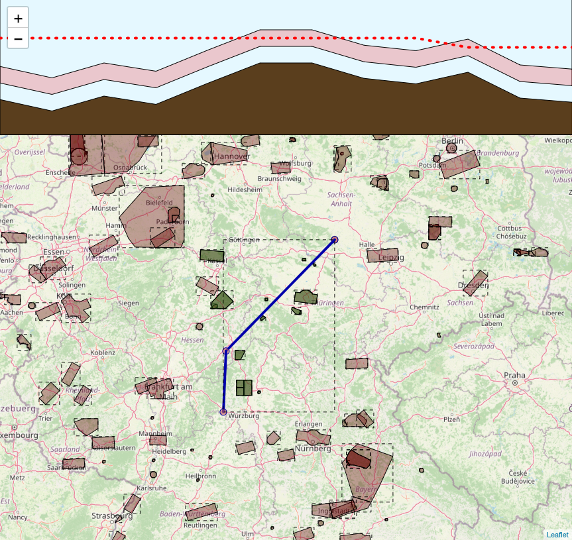
\includegraphics[width=\columnwidth]{images/final-map-with-routing-and-height-profile}
    \captionof{figure}{Visualisierung}
\end{figure}

Der Zeichenbereich setzt sich aus zwei Bereichen zusammen (Fig.6).
Im oberen Bereich der Visualisierung wird ein Höhenprofil der Route dargestellt, sowie ein Korridor, innerhalb dessen sich die Drohne bewegen darf. Dieser Korridor hängt von der Höhe der Drohne und der Bodenhöhe ab.
Im unteren Bereich befindet sich dann die interaktive Karte, auf der die Sperrzonen und die Route dargestellt werden.

Jede Route und Sperrzone ist dabei ein Array von Koordinaten, die in der Karte dargestellt werden. Routen werden in der Karte mit einem blauen Pfad dargestellt, während Sperrzonen als rote Bereiche dargestellt werden.

Diese Visualisierung war nicht direkter Bestandteil der Arbeit,  stellte sich jedoch als wichtig für die Nachvollziehbarkeit der Korrektheit der Berechnungen sowie zur Veranschaulichung und Erklärung der Vorgänge heraus.